\section{Randomiseret Min-Cut}
\subsection{Forklaring af algoritmen}

Givet en sammenhængende ikke-orienteret graf $G = (V, E)$, da er et min-cut i $G$ en kantmængde $E'$ af minimal størrelse, så $(V, E \backslash E')$ er ikke-sammenhængende.\\

Algoritmen fungerer således:
\begin{itemize}
	\item Vælg kant $e$ uniformt i $E$
	\item Contract $e$ og fjern self-loops
	\item Gentag indtil antal knuder $|V'| = 2$
	\item Returner kantmængde mellem de to knuder
\end{itemize}

\begin{figure}[H]
	\begin{center}
		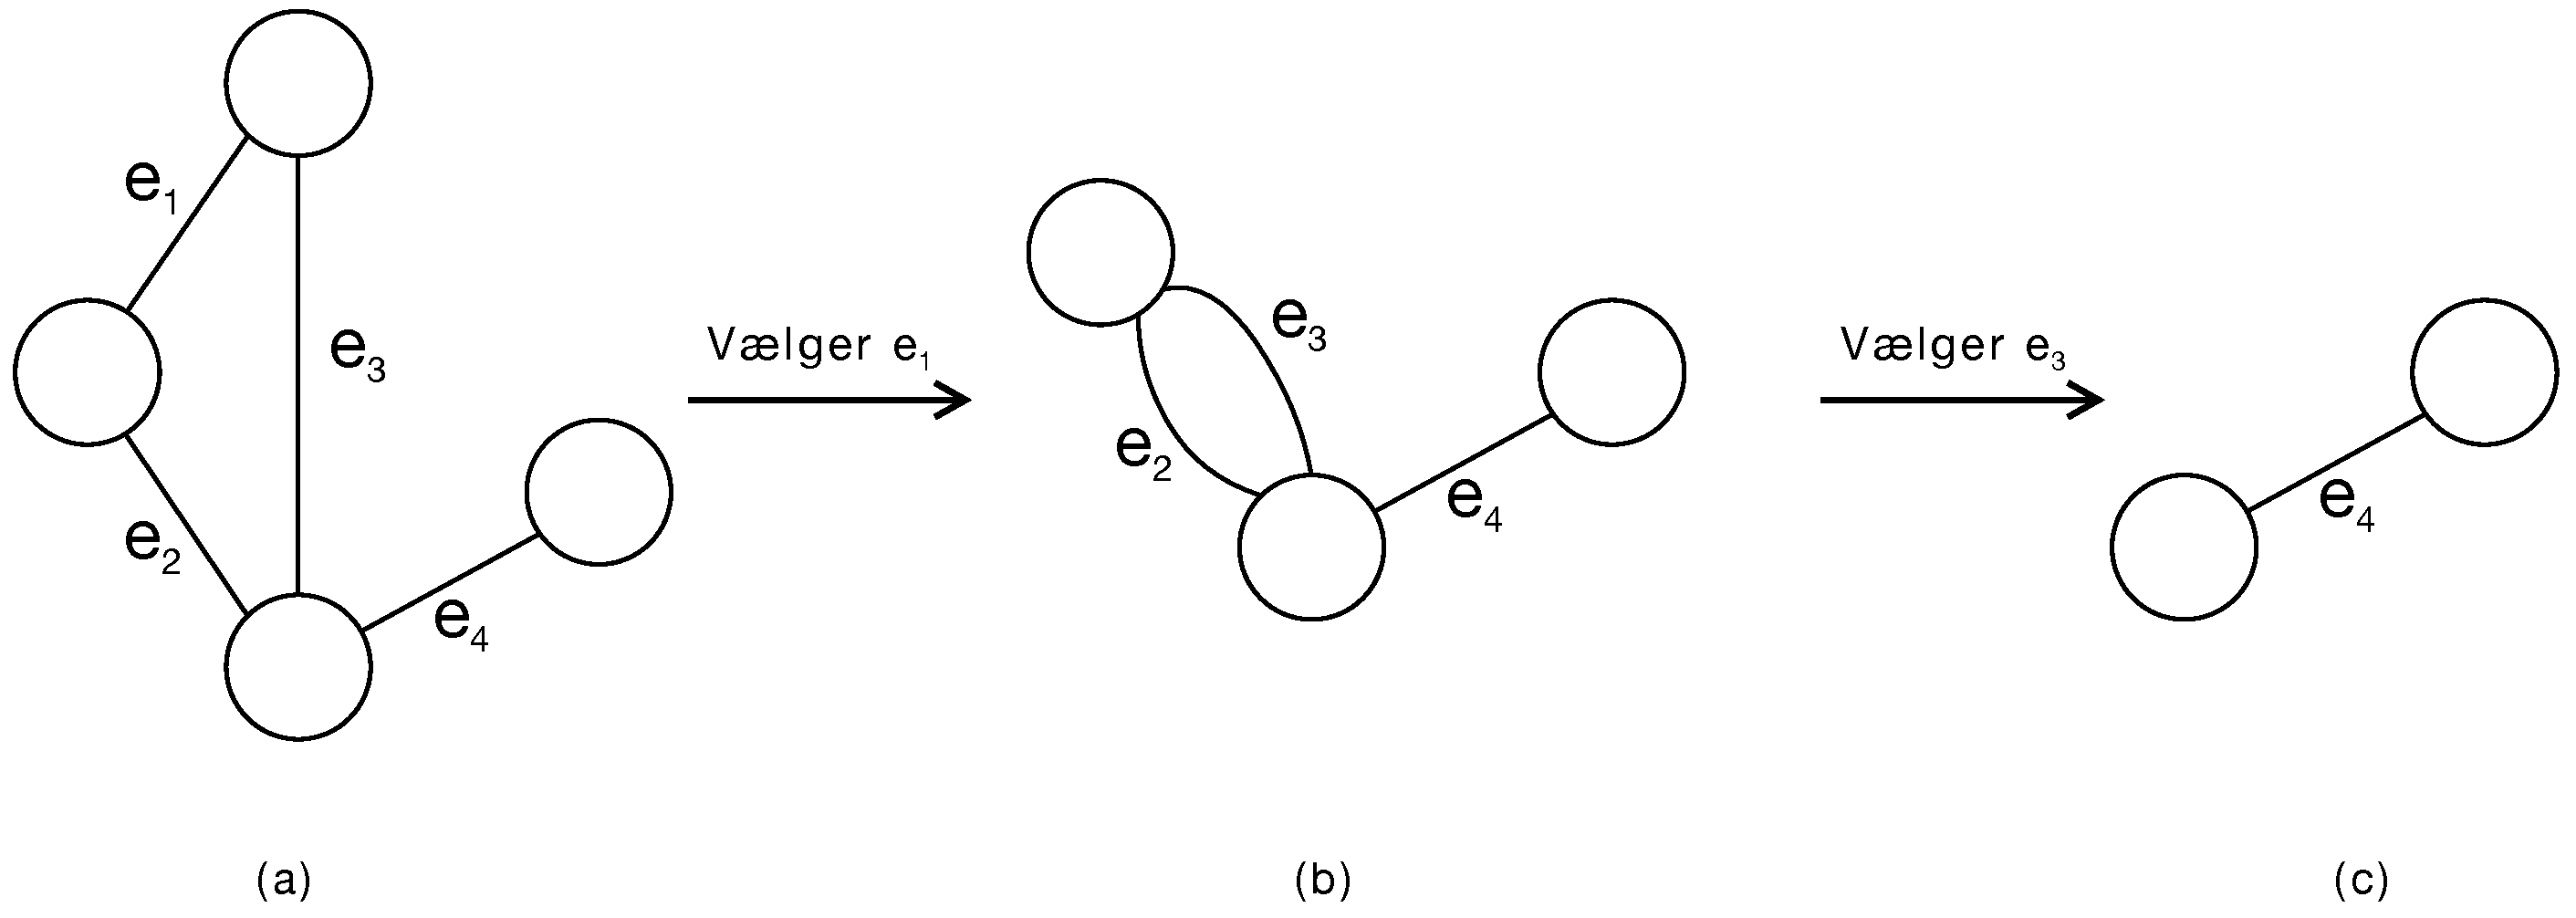
\includegraphics[width=\textwidth]{min-cut.pdf}
	\end{center}
	\caption{Eksempel på Min-Cut}
	\label{fig:min-cut}
\end{figure}

På \ref{fig:min-cut} fra (a) til (b) vælger vi $e_1$. Herved sker der en contraction. Fra (b) til (c) vælger vi $e_3$, hvorved der igen sker en contraction. Vi ser, at vi nu har et self-loop, så det fjerner vi. Nu er der kun to knuder tilbage, så algoritmen er færdig og vi returnerer kantmængden $\{e_4\}$.\\

\textbf{NB:} Bemærk at vi fra (b) til (c) potentielt godt kunne have valgt kant $e_4$, og herved ville vi ikke have fundet et min-cut.





\subsection{Sandsynlighed for succes for én iteration}
Lad os nu betragte et min-cut $C$ og lade $k$ være antallet af kanter i $C$, $k = |C|$. Lad os derudover sige, at $n = |V|$. Og lad os indføre begrebet ''degree'' for hver knude, som beskriver antal kanter der rører knuden.\\

Betragt iteration $i$ hvor $1 \leq i \leq n-2$ (dette er netop det antal iterationer algoritmen vil gå igennem, da vi stopper når der er to knuder tilbage og der fjernes en knude pr. contraction).\\


Antag, at ingen af de kanter der løbende blev contracted i $G$ i iteration $1 \, .. \, i-1$  indgår i vores optimale løsning $C$, således vi ikke potentielt får en fejlagtig løsning.\\

Da der er $n$ knuder til at starte med og der fjernes én pr. contraction, så må der efter $i-1$ iterationer være $n-i+1$ knuder i $G$.\\

Da $k = |C|$ for et min-cut $C$, så må minimum cut-størrelsen i $G$ være $\geq k$. Derfor må der altså også som minimum være $k$ kanter der rører hver knude, så $G_{\text{min\_degree}} \geq k$.\\

Da vi havde, at der var $n-i+1$ knuder i $G$, og vi lige har vist at de alle minimum har degree $k$, så kan vi få et lower bound for antal kanter $|E|$ i $G$:
\begin{align*}
|E| \geq \frac{(n-i+1)k}{2}
\end{align*}

Her dividerer vi med 2, da vi tager højde for at enhver kant $e$ vil røre to knuder.\\

Således kan vi bestemme sandsynligheden for at en af kanterne i $C$ contractes i iteration $i$ til:
\begin{align} \label{eq:prob-c}
\P[\text{En kant i $C$ contractes i iteration $i$}] = \frac{k}{|E|} \leq \frac{k}{\frac{1}{2}(n-i+1)k} = \frac{2}{n-i+1}
\end{align}
Dette gælder, da $k$ er antallet af kanter i $C$ og vi ønsker at finde sandsynligheden for at vi tilfældigt vælger en af disse kanter ud af alle kanter $|E|$.\\

Lad os nu definere eventet $\E_i$, som svarer til ''det omvendte'' af eventet beskrevet i \cref{eq:prob-c}\\
$\E_i$: Ingen kant indeholdt i $C$ vælges i iteration $i$.\\

Sandsynlighed for $\E_i$ givet succes i alle foregående iterationer kan herved beskrives som:
\begin{align} \label{eq:prob-succes-given-former-succes}
    \P \square{ \E_i \middle| \bigcap_{j=1}^{i-1} \E_j} \geq 1 - \frac{2}{n-i+1} = \frac{n-i+1-2}{n-i+1} = \frac{n-i-1}{n-i+1}
\end{align}



\subsection{Sandsynlighed for succes for én hel kørsel}

Da sandsynligheden for at algoritmen terminerer med korrekt resultat svarer til sandsynligheden for at ingen kanter i $C$ vælges i \emph{nogle som helst} af iterationerne (hvor vi tager højde for at der muligvis kan findes flere gyldige min-cut), kan vi benytte \cref{eq:prob-succes-given-former-succes} til at opskrive følgende:
\begin{align}
    \P[\text{Succes}] &\geq \P \square{ \bigcup_{i=1}^{n-2}   \E_i} \label{eq:p-succes} \\
                      &= \P[\E_1] * \P[\E_2 | \E_1] * \P[\E_3 | \E_1 \cap \E_2] \cdots \P \square{ \E_{n-2} \middle| \bigcap_{i=1}^{n-3} \E_i } \nonumber \\
                      &= \prod_{i=1}^{n-2} \P \square{ \E_i \middle| \bigcap_{j=1}^{i-1} \E_j } \nonumber \\
                      &\geq \prod_{i=1}^{n-2} \p{ \frac{n-i-1}{n-i+1} } \label{eq:indsaat-res} \\
                      &= \frac{\cancel{(n-2) \cdots 4*3}*2*1 }{n(n-1)\cancel{(n-2) \cdots 4*3} } \nonumber \\
                      &= \frac{2}{n(n-1)} \nonumber \\
                      &\geq \frac{2}{n^2} \nonumber
\end{align}

I \cref{eq:p-succes} gælder ulighedstegnet, da der muligvis findes flere gyldige min-cuts.\\
I \cref{eq:indsaat-res} indsætter vi vores resultat fra \cref{eq:prob-succes-given-former-succes}.



\subsection{Sandsynlighed for succes givet flere kørsler af algoritmen}
Vi har netop set for den randomiserede min-cut algoritme, at for én kørsel på et input med $n = |V|$, antal knuder, har vi:
$$
\P[\text{Succes}] \geq \frac{2}{n^2} \quad \Longleftrightarrow \quad \P[\text{Fejl}] \leq 1 - \frac{2}{n^2}
$$

Derudover ved vi, at følgende ulighed gælder for alle $x \in \R$:
\begin{align} \label{eq:exp-regel}
    1 + x \leq e^x
\end{align}

Lad os nu forestille os, at vi kører Min-Cut $k$ gange og returnerer det mindste cut fundet. Denne fremgangsmåde kan kun fejle hvis ingen af kørslerne finder et min-cut. Lad os for at gøre vores analyse nemmere sige vi udfører $k = n^2/2$ kørsler.

\begin{align}
    \P[\text{Fejl med $k$ kørsler}] &\leq \p{ 1 - \frac{2}{n^2} }^k \label{eq:koerer-flere-gange} \\
                                    &\leq \p{e^{- \frac{2}{n^2}}}^k \label{eq:bruger-exp-regel} \\
                                    &= e^{- \frac{2k}{n^2}} \label{eq:ganger-k-ind} \\
                                    &= e^{-1} \label{eq:benytter-vaardi-for-k} \\
                                    &\Updownarrow \nonumber \\
    \P[\text{Succes med $k$ kørsler}] &\geq 1 - e^{-1} \nonumber
\end{align}

I \cref{eq:koerer-flere-gange} ganger vi blot sandsynlighederne for at få fejl $k$ gange sammen.\\
I \cref{eq:bruger-exp-regel} benytter vi reglen i \cref{eq:exp-regel}, hvor $x = -2/n^2$.\\
I \cref{eq:ganger-k-ind} bruger vi potensregler til at sætte $k$ ind i samme potens.\\
I \cref{eq:benytter-vaardi-for-k} benytter vi, at vi sagde vi udførte $k = n^2/2$ kørsler.
